\documentclass[a4paper,11pt]{article} % screen setting

\usepackage[a4paper]{geometry}
\geometry{verbose,tmargin=1.5cm,bmargin=1.5cm,lmargin=1.5cm,rmargin=1.5cm}

\setlength{\parskip}{\smallskipamount}
\setlength{\parindent}{0pt}

%\usepackage{fontspec}
\usepackage[libertine]{newtxmath}
\usepackage[no-math]{fontspec}
\setmainfont{Linux Libertine O}
\setmonofont{DejaVu Sans Mono}

\usepackage{hyperref}
\usepackage{url}
\usepackage{xcolor}

% DARKMODE
%\pagecolor[rgb]{0,0,0} %black
%\color[rgb]{0.8,0.8,0.8} %grey

\usepackage{amsmath}
\usepackage{amssymb}

\usepackage{graphicx}
\usepackage{float}

\usepackage{minted}

\newminted{dart}{breaklines,fontsize=\footnotesize}
\newminted{bash}{breaklines,fontsize=\footnotesize}
\newminted{text}{breaklines,fontsize=\footnotesize}

\newcommand{\txtinline}[1]{\mintinline[breaklines,fontsize=\footnotesize]{text}{#1}}
\newcommand{\dartinline}[1]{\mintinline[breaklines,fontsize=\footnotesize]{python}{#1}}

\newmintedfile[pythonfile]{python}{breaklines,fontsize=\footnotesize}

\definecolor{mintedbg}{rgb}{0.90,0.90,0.90}
\usepackage{mdframed}
\BeforeBeginEnvironment{minted}{
    \begin{mdframed}[backgroundcolor=mintedbg,%
        topline=false,bottomline=false,%
        leftline=false,rightline=false]
}
\AfterEndEnvironment{minted}{\end{mdframed}}


\usepackage{setspace}

\onehalfspacing

\usepackage{appendix}


\newcommand{\highlighteq}[1]{\colorbox{blue!25}{$\displaystyle#1$}}
\newcommand{\highlight}[1]{\colorbox{red!25}{#1}}


\begin{document}


\title{Pemrograman User Interface dengan Flutter:\\
Input Widgets}
\author{Fadjar Fathurrahman}
\date{}
\maketitle

\section{Tujuan}

\begin{itemize}
\item mengenal dan menggunakan beberapa input widgets yang sering ditemukan
pada aplikasi Flutter
\end{itemize}

\section{Input Widgets}

Sebagian besar aplikasi didesain tidak hanya untuk menyampaikan atau menampilkan
informasi, namum juga berinteraksi dengan pengguna. Salah satu interaksi dengan
pengguna adalah melalui gestur (salah satunya adalah klik) dan input data seperti
yang kita temui pada form HTML.

Flutter memiliki sangat banyak input widgets yang dapat digunakan.
Pada praktikum ini kita akan mengenal beberapa
input widgets yang sering digunakan:
\begin{itemize}
\item text field
\item checkbox
\item radio button
\item slider
\item dropdown
\end{itemize}

\section{Text field}

Text field pada Flutter direpresentasikan dengan widget \txtinline{TextField}.
Contoh penggunaan:

\begin{dartcode}
TextField(
  controller: _controller,
  decoration: InputDecoration(
    labelText: 'Nama'
    hintText: 'Ketik nama Anda di sini'
  )
);
\end{dartcode}

Parameter \txtinline{controller} memiliki banyak kegunaan, salah satunya adalah
untuk menangani input dari pengguna. Contoh inisialisasi \txtinline{controller}
untuk \txtinline{TextField}:
\begin{dartcode}
final _controller = TextEditingController();
\end{dartcode}

Berikut ini adalah contoh program yang akan kita gunakan. Program ini merupakan
potongan program, Anda harus membuat membuat program utama untuk memanggil program
ini.
\begin{dartcode}
import 'package:flutter/material.dart';

class ExampleInput01 extends StatefulWidget {
  ExampleInput01({Key key}) : super(key: key);
  
  @override
  _ExampleInput01State createState() => _ExampleInput01State();
}
  
class _ExampleInput01State extends State<ExampleInput01> {
    
  final _inpNamaCtrl = TextEditingController();
  String _nama = '';
  
  void dispose() {
    _inpNamaCtrl.dispose();
    super.dispose();
  } // dispose
  
  void _handleSetNama(String inpstr) {
    setState( () {
      _nama = inpstr;
    });
  }

  Widget build(BuildContext context) {

    // TextField yang kita gunakan dibungkus dengan Container agar lebih
    // mudah untuk mengatur padding
    final inpNama = Container(
      alignment: Alignment.center,
      padding: const EdgeInsets.all(6),
      child: TextField(
        controller: _inpNamaCtrl,
        decoration: InputDecoration(
          labelText: 'Nama',
          hintText: 'Ketik nama Anda di sini',
        ),
        onChanged: _handleSetNama,
      )
    );  
    
    final outNama = Container(
      alignment: Alignment.centerLeft,
      padding: EdgeInsets.all(10),
      child: Text(
        'Anda memasukkan nama: $_nama',
        style: TextStyle(fontSize: 15,)
      ),
    );  
  
    return Scaffold(
      body: Column(
        mainAxisAlignment: MainAxisAlignment.center,
        children: [
          inpNama,
          outNama,
        ],
      )
    );
  }
}
\end{dartcode}

Contoh tampilan program:

{\centering
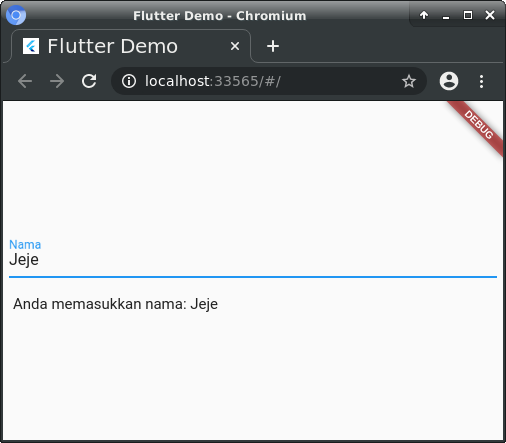
\includegraphics[scale=0.5]{images/InputNama.png}
\par}

Untuk membatasi karakter apa saja yang dapat diketikkan pada suatu \txtinline{TextField},
Anda dapat menggunakan property \txtinline{inputFormatters} dari \txtinline{TextField}.
Beberapa kelas yang dapat digunakan (built-in) pada Flutter:
\begin{itemize}
\item \txtinline{LengthLimitingTextInputFormatter}
\item \txtinline{WhitelistingTextInputFormatter}
\item \txtinline{BlacklistingTextInputFormatter}
\end{itemize}
Contoh:
\begin{dartcode}
TextField(
  inputFormatters: [
    // Hanya karakter angka, spasi, atau strip
    WhitelistingTextInputFormatter(RegExp('[0-9 -]')),
    // Panjang maksimal 16
    LengthLimitingTextInputFormatter(16),
  ]
)
\end{dartcode}


\section{Checkbox}

\txtinline{Checkbox} digunakan pada Flutter untuk mendapat input bernilai boolean.
Contoh penggunaan (dengan label):

\begin{dartcode}
Row(
  mainAxisAlignment: MainAxisAlignment.center,
  children: [
    Checkbox(
      value: _setuju,
      onChanged: _handleSetuju,
    ),
    Text('Setuju'),
  ],
);
\end{dartcode}

Variabel \txtinline{_setuju} adalah suatu variabel state pada
suatu \txtinline{StatefulWidget} dan \txtinline{_handleSetuju}
digunakan sebagai callback ketika nilai suatu \txtinline{Checkbox}
berubah.
\begin{dartcode}
bool _setuju = false;

// Callback untuk checkbox
void _handleSetuju(bool val) {
  setState( () {
    _setuju = val;
  });
}
\end{dartcode}

\section{Radio}
Widget \txtinline{Radio} biasa digunakan untuk menerima input yang berupa enumeration.
Contoh:
\begin{dartcode}

enum NilaiKepuasan { 
  baik,
  jelek,
  biasa,
}

NilaiKepuasan _nilaiKepuasan = NilaiKepuasan.baik;

final radioPuasBaik = ListTile(
  title: Text('Baik'), 
  leading: Radio(
    groupValue: _nilaiKepuasan,
    value: NilaiKepuasan.baik,
    onChanged: (NilaiKepuasan val) {
      setState( () {
        _nilaiKepuasan = val;
      });
    },
  ),
);

final radioPuasJelek = ListTile(
  title: Text('Jelek'), 
  leading: Radio(
    groupValue: _nilaiKepuasan,
    value: NilaiKepuasan.jelek,
    onChanged: (NilaiKepuasan val) {
      setState( () {
        _nilaiKepuasan = val;
      });
    },
  ),
);

final radioPuasBiasa = ListTile(
  title: Text('Biasa'), 
  leading: Radio(
    groupValue: _nilaiKepuasan,
    value: NilaiKepuasan.biasa,
    onChanged: (NilaiKepuasan val) {
      setState( () {
        _nilaiKepuasan = val;
      });
    },
  ),
);
\end{dartcode}

Contoh tampilan:

{\centering
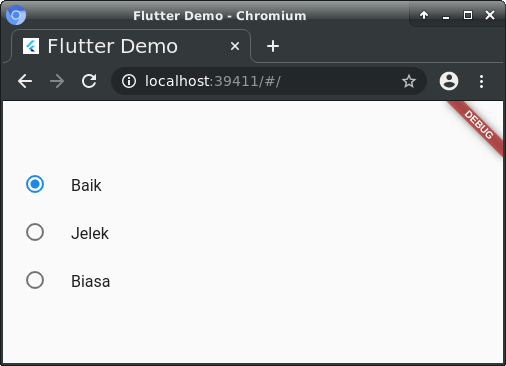
\includegraphics[scale=0.5]{images/RadioBox1.png}
\par}


\section{Slider}

\txtinline{Slider} biasa digunakan untuk menampilkan nilai numerik.
Contoh:
\begin{dartcode}
double _nilaiSlider = 0;

final sliderNilai = Slider(
  label: _nilaiSlider.toString(),
  min: 0, max: 100,
  divisions: 100,
  value: _nilaiSlider,
  onChanged: (double val) {
    setState( () {
      _nilaiSlider = val;
    });
  }
);
\end{dartcode}

Contoh tampilan:

{\centering
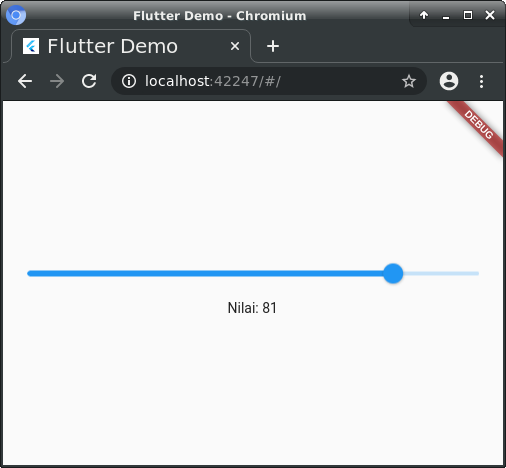
\includegraphics[scale=0.5]{images/SliderDouble1.png}
\par}


\section{Dropdown}

Kegunaan widget ini mirip dengan \txtinline{Radio}.
Contoh penggunaan:
\begin{dartcode}
final db1 = DropdownButton<NilaiKepuasan>(
  value: _nilaiKepuasan,
  items: const <DropdownMenuItem<NilaiKepuasan>>[
    DropdownMenuItem<NilaiKepuasan>(
      child: Text('Baik'),
      value: NilaiKepuasan.baik,
    ),
    DropdownMenuItem<NilaiKepuasan>(
      child: Text('Jelek'),
      value: NilaiKepuasan.jelek,
    ),
    DropdownMenuItem<NilaiKepuasan>(
      child: Text('Biasa'),
      value: NilaiKepuasan.biasa,
    ),
  ],
  onChanged: (NilaiKepuasan val) {
    setState( () {
      _nilaiKepuasan = val;
    });
  },
);
\end{dartcode}

Contoh tampilan:

{\centering
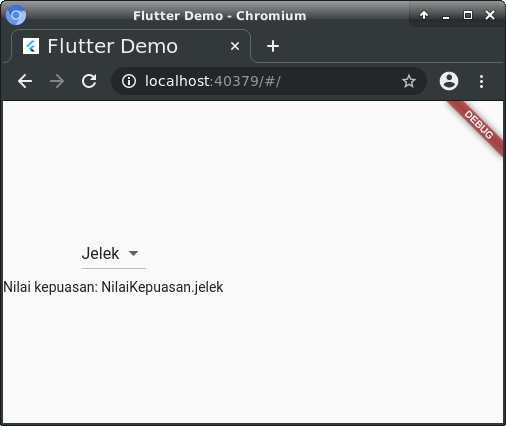
\includegraphics[scale=0.5]{images/dropdown1.png}
\par}

\section{Tugas}
Lengkapi potongan program di atas sehingga dapat menjadi program Flutter yang
dapat dijalankan.


\bibliographystyle{unsrt}
\bibliography{BIBLIO}

\end{document}
